
    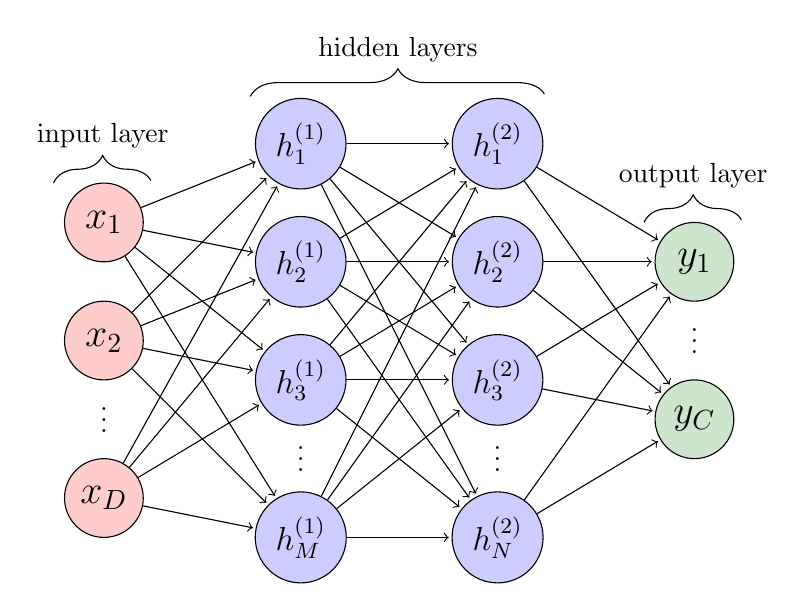
\begin{tikzpicture}[shorten >=1pt]
	\tikzstyle{unit}=[draw,shape=circle,minimum size=1.0cm]
	
	%\node[unit,fill=red!20](x1) at (0,5.0){\Large $x_1$};
	\node[unit,fill=red!20](x1) at (0,3.5){\Large $x_1$};
	\node[unit,fill=red!20](x2) at (0,2){\Large $x_2$};
	\node(dots) at (0,1.1){\vdots};
	\node[unit,fill=red!20](xd) at (0,0){\Large $x_D$};
	
	%\node[unit,fill=blue!20](w11) at (2.5,6.0){\large $h_1^{(1)}$};
	\node[unit,fill=blue!20](h11) at (2.5,4.5){\large $h_1^{(1)}$};
	\node[unit,fill=blue!20](h12) at (2.5,3.0){\large $h_2^{(1)}$};
	\node[unit,fill=blue!20](h13) at (2.5,1.5){\large $h_3^{(1)}$};
	\node(dots) at (2.5,0.6){\vdots};
	\node[unit,fill=blue!20](h1m) at (2.5,-0.5){\large $h_M^{(1)}$};
	
	%\node[unit,fill=blue!20](w21) at (5,6.0){\large $h_1^{(2)}$};
	\node[unit,fill=blue!20](h21) at (5,4.5){\large $h_1^{(2)}$};
	\node[unit,fill=blue!20](h22) at (5,3.0){\large $h_2^{(2)}$};
	\node[unit,fill=blue!20](h23) at (5,1.5){\large $h_3^{(2)}$};
	\node(dots) at (5,0.6){\vdots};
	\node[unit,fill=blue!20](h2n) at (5,-0.5){\large $h_N^{(2)}$};
	
	%\node[unit,fill=green!20](y1) at (7.5,4.5){\Large $y_1$};
	\node[unit,fill=Green!20](y1) at (7.5,3.0){\Large $y_1$};
	\node(dots) at (7.5,2.1){\vdots};
	\node[unit,fill=Green!20](yc) at (7.5,1.0){\Large $y_C$};
	
	% input to hidden1
	\draw[->] (x1) -- (h11);
	\draw[->] (x1) -- (h12);
	\draw[->] (x1) -- (h13);
	%\draw[->] (x1) -- (h14);
	\draw[->] (x1) -- (h1m);
	
	\draw[->] (x2) -- (h11);
	\draw[->] (x2) -- (h12);
	\draw[->] (x2) -- (h13);
	%\draw[->] (x2) -- (h14);
	\draw[->] (x2) -- (h1m);
	
	%\draw[->] (x3) -- (h11);
	%\draw[->] (x3) -- (h12);
	%\draw[->] (x3) -- (h13);
	%\draw[->] (x3) -- (h14);
	%\draw[->] (x3) -- (h1m);
	
	\draw[->] (xd) -- (h11);
	\draw[->] (xd) -- (h12);
	\draw[->] (xd) -- (h13);
	%\draw[->] (xd) -- (h14);
	\draw[->] (xd) -- (h1m);
	
	% hidden1 to hidden2
	\draw[->] (h11) -- (h21);
	\draw[->] (h11) -- (h22);
	\draw[->] (h11) -- (h23);
	%\draw[->] (h11) -- (h24);
	\draw[->] (h11) -- (h2n);
	
	\draw[->] (h12) -- (h21);
	\draw[->] (h12) -- (h22);
	\draw[->] (h12) -- (h23);
	%\draw[->] (h12) -- (h24);
	\draw[->] (h12) -- (h2n);
	
	\draw[->] (h13) -- (h21);
	\draw[->] (h13) -- (h22);
	\draw[->] (h13) -- (h23);
	%\draw[->] (h13) -- (h24);
	\draw[->] (h13) -- (h2n);
	
	%\draw[->] (h14) -- (h21);
	%\draw[->] (h14) -- (h22);
	%\draw[->] (h14) -- (h23);
	%\draw[->] (h14) -- (h24);
	%\draw[->] (h14) -- (h2n);
	
	\draw[->] (h1m) -- (h21);
	\draw[->] (h1m) -- (h22);
	\draw[->] (h1m) -- (h23);
	%\draw[->] (w1m) -- (h24);
	\draw[->] (h1m) -- (h2n);
	
	% hidden2 to output
	\draw[->] (h21) -- (y1);
	%\draw[->] (h21) -- (y2);
	\draw[->] (h21) -- (yc);
	
	\draw[->] (h22) -- (y1);
	%\draw[->] (h22) -- (y2);
	\draw[->] (h22) -- (yc);
	
	\draw[->] (h23) -- (y1);
	%\draw[->] (h23) -- (y2);
	\draw[->] (h23) -- (yc);
	
	%\draw[->] (h24) -- (y1);
	%\draw[->] (h24) -- (y2);
	%\draw[->] (h24) -- (yc);
	
	\draw[->] (h2n) -- (y1);
	%\draw[->] (h2n) -- (y2);
	\draw[->] (h2n) -- (yc);
	\draw [decorate,decoration={brace,amplitude=10pt},xshift=-4pt,yshift=0pt] (-0.5,4.0) -- (0.75,4.0) node [black,midway,yshift=+0.6cm]{input layer};
	\draw [decorate,decoration={brace,amplitude=10pt},xshift=-4pt,yshift=0pt] (2.0,5.1) -- (5.75,5.1) node [black,midway,yshift=+0.6cm]{hidden layers};
	\draw [decorate,decoration={brace,amplitude=10pt},xshift=-4pt,yshift=0pt] (7.0,3.5) -- (8.25,3.5) node [black,midway,yshift=+0.6cm]{output layer};
\end{tikzpicture}